\chapter[Amenity]{Incorporating amenity - non monetary income}\label{appendix-amenity}
% from Ricardo_Rent_and_Roemer_3.tex
% We will also include an urban wage premium. Otherwise the amenity factor is the only attractor. The wage premium provides a reason to travel to the city centre. The literature supports the notion that there is an  urban wage premium.  We will consider later how the premium arises from agglomeration externalities in production. 


Basic New Economic Geography models posit two centripetal forces: households' preference for variety in the consumer goods they can buy; and economies of scale in manufacturing (\cite{gurwitzCatastrophicAgglomeration2019}).\footnote{In NEG models the variety of consumption goods comes from specifying production sectors in which larger markets support more variety.} We will deal first with the first of these.  A simple way to incorporate agglomeration amenities is to include what might be called a `utility premium' for urban dwellers  as non-monetary location income 
$A(d; n), \die{a}{n}\leq 0)$ depending on distance, $d$ from the centre and population $n$, A simple linear  function representing the utility premium on location is convenient for illustration:
\begin{equation}
U(w,d)= w+ \omega+ A(d; n) - T(d))
\label{eqn-u}
\end{equation}
where $w$  is an urban wage premium, $T(d)$ is transportation cost from the centre to $d$.
\footnote{\cite{anasUrbanSpatialStructure1998} show that a linear transportation cost will not  hold if congestion declines  with $d$.} %and $H(d)$ is the physical house cost independent of land value at $d$. WE assume 

What we call the `wage premium' is simply the urban wage in most models.  In the most common versions of the model there is no amenity and there is no wage outside of the city limits, but there may be a land cost. In our model the wage premium will result from agglomeration economies in production.
A linear amenity function, for example $A(d|n)= a-b*d$, is convenient to illustrative purposes.  It will allow simple experiments with the effect of  increasing population on city size, wages and rents. 

%\footnote{wage income, if all income goes to housing, or the share of wage income going to housing services.   (If we use a Cobb-Douglas utility function we would just replace $w$ with    $\alpha Y$, where $Y$ is household income and $\alpha$ is the share of total income. } Let  $T(d)=td$ be transportation cost with  $t>0$. 

We employ the standard equilibrium assumption, \[ U^{urban}(w+\omega, d)=U^{alternative}(\omega), \forall  d\] 
%This simple model ignores that there might be a land cost a outside of the city. %The simplest way to think about the model is to \textbf{treat w as a wage premium for working in the city}. 
In a migration equilibrium, land rent rises to absorb all of the utility premium. This model endogenizes the city size for a given wage premium. 



\begin{figure}[htbp]
\begin{center}
%
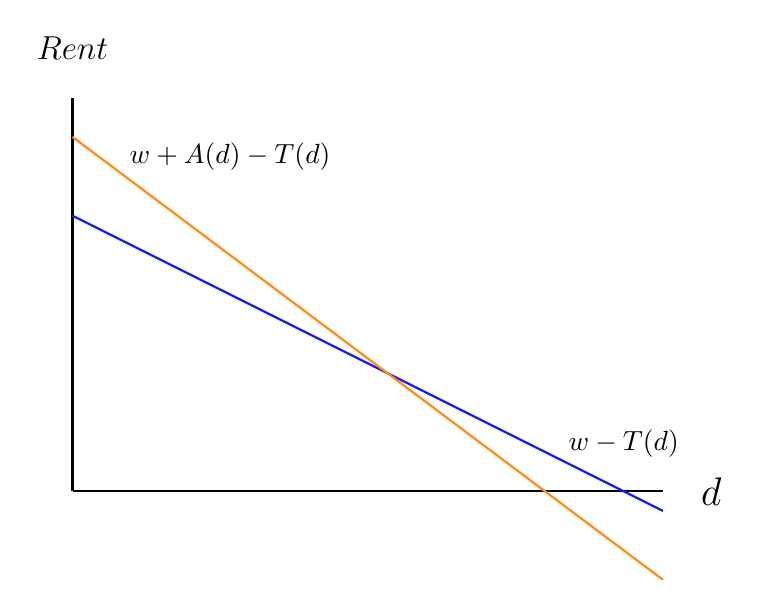
\begin{tikzpicture}[scale=.5]
\def\bndmax{5}        %https://tex.stackexchange.com/questions/68462/filling-a-complex-region-with-tikz
\def\bndmin{0.2}
\def \n {10}
\def \m {15}
\def \t {.5}
\def \th {1}
\def \w {7}
\tikzset{func/.style={thick,color=blue!90}}	
\draw [thick] (0,\n)node[above=10]{\large$Rent$}--(0,0);
\draw [thick] (0,0)--(\m,0)node[right=10]{\Large $d$};
%\foreach \xi in {0,..., \m} \draw (\xi,0)--(\xi,-.1)node[below=1]{\small$\xi$};
%\foreach \yi in {1,...,\n} \draw (0,\yi)--(-.1,\yi)node[left]{$\yi$};
%%\foreach \i in {1,4,9,16} {
	\draw[func,domain=0:\m] plot [samples=200] (\x,{\w-\t*\x});
%	\draw[func,domain=0:\m, dashed] plot [samples=200] (\x,{\w+\azero-\th*\x+\aprime*\x});

\node at (14,1.2){$w-T(d)$};
\def \azero{2}
\def \aprime {-.25}	
\tikzset{func/.style={thick,color=orange!90}}	
	\draw[func,domain=0:\m] plot [samples=200] (\x,{\w+\azero-\t*\x+\aprime*\x});
\node at (4,8.5){$w +A(d)-T(d)$};
%\node at(-.8,2) [left]{base $2^1=$};
%\node at(-.8,1) [left]{$2^0=$};
%\draw[dotted] (0,2)--(1,2)--(1,0); 
 \end{tikzpicture}

\caption{Rent profile with amenities}
\label{fig-amenity1}
\end{center}
\end{figure}

 If $A=0$ and $T=td$,  \ref{eqn-u} this model produces the standard result in the Alonzo model (land rent declining linearly with distance) as the blue line in Figure~\ref{fig-amenity1} shows.
 \footnote{The very simple results rests on several assumptions - no other housing expense, housing all the same size, wages all equal, preferences identical, transportation costs.}  The triangle below the line is the rent accruing to landowners.

In the familiar version of the model there is no amenity and there is no wage outside of the city limits.
What we call the wage premium is simply the urban wage in simple models. A model with amenity declining with $d$ and no transportation cost would produced the  standard result. 

If $A(0)>0$, willingness to pay and therefore the competitive rent profile is like the orange line.  
  
The  higher rent comes not from a housing budget but from household demand for amenity.  Housing choice is always the purchase of  a bundle of characteristics such as location, building space, yard, local density and local amenities.  We are holding features of the housing constant and adding an explicit urban amenity which is not available in other locations and may be provided at a different level in other cities.  Households outside of the city will purchase a different amenity---perhaps a larger yard or house, quiet,  trees, or leisure. 
  
  \textbf{Rent will be higher at the centre of a city with higher amenity}.   
    
 % \textbf{A city with higher amenity may have a lower equilibrium wage.} (When will this occur?)
   
If  amenity goes below zero in the outer regions of the city as illustrated by the orange line  in Figure~\ref{fig-amenity1}, the geographical size of the  city will be smaller.  With  linear functions this happens if $\frac{a}{b} < \frac{w}{t}$. There would be a band of land around the city with negative amenity. 
  
The far more likely case is that $A(d) > 0$ when $w-T(d)$ falls to zero. In this case there is a band of  residents around the city, outside of the population commuting to work. They do not travel to work,  do not collect a wage, but still enjoy the amenity of being close to a city. This might be a population of retired persons enjoying occasional visits and health-care facilities.




%Agglomeration amenity is likely to raise wages outside of the city though competition if the overall labour supply is fixed and labour is used outside of the city.

Since employers will not pay for the amenity, some amenities may be financed publicly. It is common to introduce the cost of generating amenities as a tax on residents. Publicly financed amenities, however, may work as a wage subsidy,  	

\section{Rent}
In Figure~\ref{fig-amenity1}, the height of the orange line above $\omega$ represents the rental value of a property at $d$, which is 
\begin{equation}
Rent(d)  =  w  + A(d) - T(d)	
\label{eqn-rent-at-d}\end{equation}
 and the area under the orange line represents the total rent collected.
 \footnote{The cost of transportation is a real cost, but the decline in amenity with distance is not.}
 
 If we solve $w-T(d)=0$ for $d$, we get the maximum  distance workers will commute, $c^{max}$. 
If we solve $w+A(d)-T(d)=0$ for $d$, we get the maximum  distance at which living near the city offers an advantage, $d^{max}$. For analytical convenience let's assume amenity and transportation are both linear functions of $d$:
\begin{eqnarray}
w+ a_0 - b*d^{max} - t*{max}  	&=0		\nonumber \\
w+a_0 - (b+t)d^{max}  	&=0			\nonumber \\
d^{max}				&= \frac{w+a_0}{b+t}
\end{eqnarray}
For the case of a circular city the area within this radius is $\pi \left(\frac{w+a_0}{b+t}\right)^2$ 



\section{Sort}
{MOVE TO FUTURE WORK/MENTION AMENITY APPENDIX? If the city generates additional social amenities\index{amenities} not captured in the wage  the money available for housing does not change, although willingness to pay must be higher. The most likely adjustments are in urban `subsistence' and it is probably offset by rural amenity that is given up to live in the city. In the long run urban amenities must exert upward pressure on rural amenities.} % These interesting extension will not be taken up in this thesis.}
